\documentclass{article}
\usepackage{bookmark}

\usepackage[utf8]{inputenc}
\usepackage[brazil]{babel}  % Define o idioma para português do Brasil
\usepackage{csquotes}       % Para lidar com aspas de maneira apropriada com babel
%\usepackage{ragged2e}       % Pacote para justificação

\usepackage{amsmath}
\usepackage{xcolor}
\usepackage{listings}
% Configuração do estilo de código
\lstset{
  language=C,
  %basicstyle=\ttfamily\footnotesize,
  keywordstyle=\color{blue},
  commentstyle=\color{gray},
  stringstyle=\color{red},
  breaklines=true,
  frame=single,
  numbers=left,
  numberstyle=\tiny,
  numbersep=5pt,
  showstringspaces=false,
}


\usepackage{graphicx}       % Pacote para inserção de imagens

\usepackage{hyperref}       % Pacote para links clicáveis
\hypersetup{
    colorlinks=true,
    linkcolor=blue,
    urlcolor=blue,
}

\usepackage{enumitem}       % Pacote para personalização de listas

\usepackage{geometry}       % Pacote para ajustar margens

\geometry{                  % Definindo margens personalizadas (em centímetros)
  left=2.5cm,  % Margem esquerda
  right=2.5cm, % Margem direita
  top=2.5cm,   % Margem superior
  bottom=2.5cm % Margem inferior
}

\usepackage[backend=biber,style=ieee]{biblatex}     % Estilo ieee para bibliografia numerada
\addbibresource{ref.bib}                            % Arquivo .bib


\begin{document}

\begin{titlepage}
    \centering
    % Cabeçalho personalizado
    
\includegraphics[width=0.3\textwidth]{../../Topic1/Avaliativo/Imagens/Logo UFLA - Colorida chapada.png}

    \vspace*{2cm} % Espaçamento vertical antes do cabeçalho
    \Large
    Universidade Federal de Lavras\\
    PPGCC\\
    PCC508 – Sistemas Operacionais\\
    
    \vspace{2cm} % Espaço entre o cabeçalho e o título
    \huge % Define o tamanho da fonte do título
    \textbf{Tópico 4 Lista Avaliativa}
    
    \vfill % Adiciona um espaçamento flexível antes do rodapé (opcional)
    
    % Opcionalmente, você pode incluir seu nome e a data aqui
    \large
    Douglas Aquino T. Mendes\\
    \today % Insere a data atual
\end{titlepage}

\tableofcontents
\newpage

\section{Introdução}
Este documento tem como objetivo apresentar o desenvolvimento das atividades avaliativas para o tópico 4 da disciplina de Sistemas Operacionais, focando na implementação de códigos em linguagem C. Serão apresentadas as questões, a resolução, os códigos desenvolvidos, seguidos de uma explicação sobre sua lógica de funcionamento.

\section{Questões}
\subsection{Memória virtual}

\textbf{Pergunta:} 1) Explique como funciona a memória virtual, juntamente com a paginação. \newline

\textbf{Resposta:}A memória virtual é um mecanismo de gerenciamento de memória que permite que os sistemas operacionais utilizem mais memória do que a fisicamente disponível no hardware (RAM). Ela faz isso mapeando endereços virtuais usados pelos programas em endereços físicos na RAM. Quando um programa tenta acessar um endereço de memória que não está na RAM, o sistema operacional interrompe o processo e carrega os dados necessários da memória secundária (geralmente o disco rígido ou SSD) para a RAM. Esse processo é chamado de page fault.
\textbf{A paginação} é uma técnica de implementação da memória virtual que divide tanto a memória virtual quanto a memória física em blocos de tamanho fixo chamados páginas e molduras de página (ou frames). Cada página virtual de um processo pode ser mapeada para uma moldura de página na RAM \cite{tanenbaum2021,escolaLBK2024}.
\begin{itemize}
    \item  A memória virtual de um processo é dividida em páginas de tamanho fixo.
    \item Cada processo tem sua própria tabela de páginas, que mapeia as páginas virtuais para as molduras físicas na RAM. Essa tabela contém informações sobre onde uma página virtual está armazenada na memória física.
    \item  Quando um programa acessa um endereço de memória virtual, a Unidade de Gestão de Memória (MMU) traduz esse endereço em um endereço físico usando a tabela de páginas.
    \item Se a página que está sendo acessada não está na RAM, ocorre um page fault. O sistema operacional pausa a execução do processo, busca a página necessária no disco e a carrega em uma moldura livre da RAM. Se não houver molduras livres, uma página existente é removida (muitas vezes usando algoritmos como LRU – Least Recently Used), e a nova página é carregada.
\end{itemize}

\subsection{Tradução de um endereço virtual}

\textbf{Pergunta:} 2) Explique em detalhes como funciona a tradução de um endereço virtual para o endereço físico em um sistema com memória virtual e paginação. Use um exemplo e considere que o endereço virtual tem mais bits que o endereço físico. Isso é possível? Explique também qual a função da MMU. \newline

\textbf{Resposta:}A memória virtual é dividida em páginas de tamanho fixo, e a memória física é dividida em molduras de página de mesmo tamanho. A tradução do endereço virtual para o endereço físico envolve o uso de uma tabela de páginas que mapeia cada página virtual para uma moldura física.

Um endereço virtual pode ser dividido em duas partes, Número da página virtual e Deslocamento (Indica a posição específica dentro da página). Um endereço físico também é dividido em duas partes, Número da moldura física e Deslocamento. Considerando um exemplo onde o endereço virtual tem 16 bits, o endereço físico tem 14 bits e o tamanho de cada página é de 1 KB, então o deslocamento dentro da página tem 10 bits, os bits restantes do endereço virtual (16 - 10 = 6 bits) representam o número da página virtual. Da mesma forma, os bits restantes do endereço físico (14 - 10 = 4 bits) representam o número da moldura física \cite{tanenbaum2021, resumosLEIC, gomesAula18}.\newline

\textbf{Exemplo de Tradução de Endereço}\newline

Considere um endereço virtual de 16 bits: 0011 1010 0101 1100.
\begin{itemize}
    \item \textbf{Número da página virtual (VPN):} Os 6 bits mais significativos → 001110.
    \item \textbf{Deslocamento: }Os 10 bits menos significativos → 101011100.
\end{itemize}

Para traduzir esse endereço, a MMU faz o seguinte:

\begin{itemize}
    \item \textbf{Consulta a tabela de páginas} usando a VPN 001110 para encontrar a moldura de página correspondente.
    \item Substitui a VPN pelo PFN obtido na tabela de páginas, mantendo o deslocamento inalterado.
    \item Suponha que a tabela de páginas indique que a VPN "001110" corresponde à PFN "0101". Então, o endereço físico resultante seria \textbf{0101} 1010 1110 1100.\newline
\end{itemize}

\textbf{A MMU} é o componente de hardware responsável por:

\begin{itemize}
    \item Converter endereços virtuais em endereços físicos em tempo real.
    \item Verificar permissões (leitura, escrita, execução) para garantir que os processos não acessem memória de forma indevida.
    \item Se a MMU não encontrar uma entrada válida na tabela de páginas (indicando que a página não está na RAM), ela aciona um page fault e chama o sistema operacional para carregar a página da memória secundária.
\end{itemize}

\subsection{Tabela de páginas}

\textbf{Pergunta:} 3) Explique a estrutura de uma tabela de páginas. \newline

\textbf{Resposta: }A tabela de páginas é uma estrutura de dados que implementam memória virtual e paginação. Sua função é mapear endereços virtuais (utilizados pelos processos) para endereços físicos (localizados na RAM). A tabela de páginas é composta por entradas, e cada entrada da tabela de páginas (Page Table Entry - PTE) contém informações sobre o mapeamento de uma página virtual para uma moldura física. Alguns componentes comuns de uma entrada de Tabela de Páginas são\cite{tanenbaum2021, profMoraesGerenciamento}:

\begin{itemize}
    \item Número da moldura física.
    \item Bit de presença.
    \item Bits de controle de acesso.
    \item Bit de modificado.
    \item Bit de referenciado.
\end{itemize}

\subsection{TLB}

\textbf{Pergunta:} 4) Explique o que é, para que serve e como funciona uma TLB (translation lookaside buffer). \newline

\textbf{Resposta:} A TLB é uma pequena, mas muito rápida, cache que armazena pares de mapeamentos de endereços virtuais e físicos. Como as operações de busca e tradução de endereços em tabelas de páginas na RAM podem ser demoradas, a TLB melhora o desempenho armazenando as traduções mais recentes. Se a MMU encontrar o mapeamento desejado na TLB, a tradução ocorre instantaneamente. A TLB é usada para Aumentar a velocidade de tradução de endereços, diminuindo o tempo de acesso à memória e  evitando acessos repetidos à tabela de páginas armazenada na RAM \cite{tanenbaum2021, techtargetTLB}.

\section{Desenvolver um programa}

\subsection{Compartilhar uma área de memória criada com a chamada mmap}
\textbf{Enunciado:} Deve ser desenvolvido um programa que cria dois processos filhos. Esses processos devem compartilhar uma área de memória criada com a chamada mmap. Vamos agora utilizar essa área como um buffer compartilhado. Um dos processos será um produtor e deve gerar uma letra aleatória em cada intervalo de tempo (configurável) e adicionar ao buffer. O outro processo deve consumir esses itens (letras), uma a cada intervalo de tempo (configurável) e imprimir o item na tela. Não esquecer o problema da condição de corrida. O processo pai não executa nenhuma tarefa, fica bloqueado esperando os processos filhos. \newline

\subsection{Código}
\label{sub-sec-cod}
\lstinputlisting[language=C]{Codes/atv1_sharedmem.c}
\subsection{Testes e Resultados}
Como resultado da execução do código exibido na subceção \ref{sub-sec-cod}, obtivemos a saída ilustrada na figura \ref{fig:exec}. É importante ressaltar que o programa pode apresentar um problema, pois não há verificação de produzir apenas quando há espaço, ou seja, o buffer pode acabar sendo subscrito pela função de produzir, antes da função de consumir. 

\begin{figure}[ht]
    \centering
    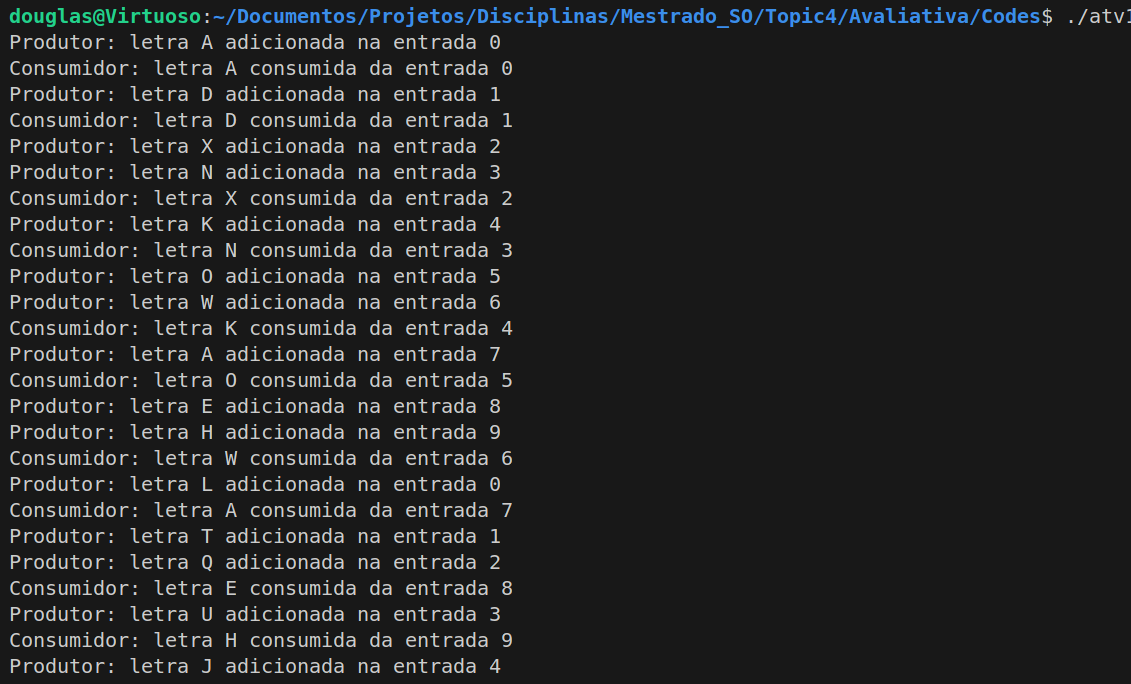
\includegraphics[width=1\textwidth]{./Images/image.png}
    \caption{Resultado da execução do programa}
    \label{fig:exec}
\end{figure}

\printbibliography % Imprime a lista de referências


\end{document}